\documentclass[tikz,border=5]{standalone}
\usepackage[utf8]{inputenc}

\usepackage{tikz}
\usetikzlibrary{positioning}
\usetikzlibrary{decorations.text}

\begin{document}


%------------------------------------------------------------------------------
%Introductory example
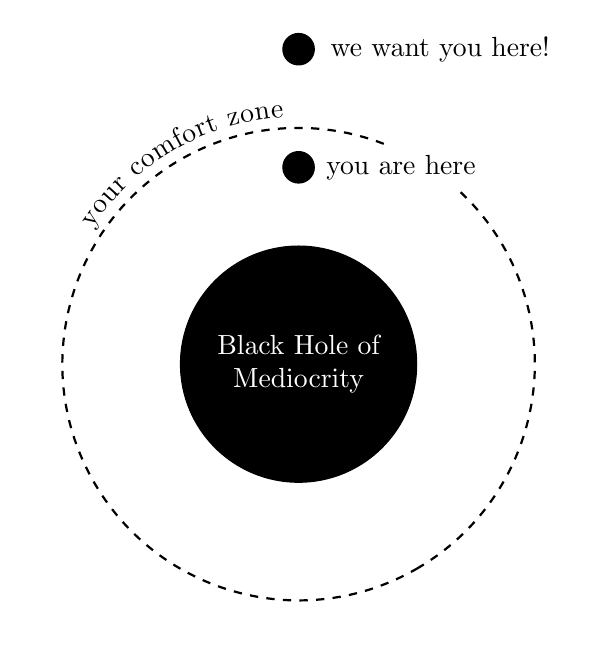
\begin{tikzpicture}  
\filldraw[black] (0,0) circle (1.5cm);
\filldraw[black] (0,2.5) circle (0.2cm);
\filldraw[black] (0,4) circle (0.2cm);
\draw (0,0) node [text width=2.5cm,align=center,color=white] {Black Hole of Mediocrity}; 
\draw[thick,dashed,-latex,black,rotate=-60,postaction={decorate},decoration={text along path,
text={your comfort zone},text align=center,reverse path,raise=4pt}]
(0,0) circle (3.0cm);

\node at (1.3,2.5) [black,fill=white]  {you are here} ;
\node at (1.8,4) [black,fill=white]  {we want you here!} ;

\end{tikzpicture}
%-----------------------------


\end{document}